\documentclass[conference]{IEEEtran}
\IEEEoverridecommandlockouts
\usepackage{cite}
\usepackage{amsmath,amssymb,amsfonts}
\usepackage{algorithmic}
\usepackage{graphicx}
\usepackage{textcomp}
\usepackage{xcolor}
\usepackage{tikz}
\usetikzlibrary{shapes.geometric, arrows.meta, positioning, calc, fit, backgrounds}
\usepackage{listings}
\renewcommand{\lstlistingname}{Code Snippet}
\usepackage{url}

\begin{document}

\title{Real-Time Quantum-Inspired 5D K-Means Image Segmentation}

\author{\IEEEauthorblockN{Sebastian Șoptelea}
\IEEEauthorblockA{\textit{Centre for the Study of Complexity} \\
\textit{Babeș-Bolyai University}\\
Cluj-Napoca, Romania \\
sebastian.soptelea1@stud.ubbcluj.ro}
}

\maketitle

\begin{abstract}
This document summarizes the development and evaluation of a high-throughput GPU-accelerated 5D K-Means image segmentation framework that compares a classical Euclidean distance metric against a quantum-inspired state overlap emulation.

\end{abstract}

\begin{IEEEkeywords}
GPU Acceleration, 5D K-Means, Quantum-Inspired Computing, SWAP Test, Real-Time Video Segmentation
\end{IEEEkeywords}

\section{Introduction}\label{sec:intro}
Image segmentation is a fundamental computer vision task that partitions an image into meaningful, uniformly connected regions \cite{gonzalez2009digital}. It is a key preprocessing step for high-level computer vision applications, such as lane-tracking in autonomous vehicles \cite{janai2020computer}, object detection \cite{redmon2016you}, and medical imaging overlays \cite{pham2000current}. While simple color-based segmentation is common, modern real-time applications require spatial consistency. To achieve this, each pixel is mapped to a 5D feature manifold:
\begin{equation}
\mathbf{x} = [B, G, R, x, y]^T
\end{equation}
By clustering pixels within this combined color-spatial manifold, the algorithm naturally groups pixels that are both chromatically similar and geometrically close, preventing pixel-level noise \cite{achanta2012slic}.

Real-time video processing places strict constraints on execution latency. In computer vision, standard real-time throughput is governed by the human-facing display refresh rate of 60 frames per second (FPS) ($16.67\text{ ms}$ per frame) \cite{DHANANI20135}. Yet, for high-speed interactive systems, including driving simulators \cite{cruden2019simulator}, virtual reality headsets \cite{jerald2009scene}, and autonomous vehicle obstacle avoidance, the standard target is high-speed real-time processing operating at $120\text{ FPS}$ or more ($8.33\text{ ms}$ or less per frame) to prevent feedback loop delays and tracking oscillation \cite{cruden2019simulator, jerald2009scene}. Running heavy deep-learning segmentation models on embedded edge devices is often impossible under these extreme limits due to massive power consumption and high latency \cite{paszke2016enet}. Therefore, highly optimized, lightweight, Graphics Processing Unit (GPU)-accelerated classical clustering is a practical alternative for edge devices \cite{farivar2008parallel}.

Simultaneously, quantum-inspired computing offers a practical model for simulating quantum mechanics on classical hardware. True quantum computers are still in the Noisy Intermediate-Scale Quantum (NISQ) era \cite{preskill2018quantum}, characterized by small physical qubit registers, lack of error correction, and short coherence times ($T_1, T_2$) \cite{bharti2022noisy}. Physical hardware is highly sensitive to environmental noise, and transferring live video frames to a Quantum Processing Unit (QPU) introduces massive network latency, rendering genuine quantum hardware unusable for real-time video \cite{fraunhofer2025quantum}. To bypass these hardware constraints while leveraging quantum mathematical behaviors, quantum-inspired computing translates quantum mechanics such as state-overlap fidelity via the SWAP test \cite{buhrman2001quantum} (which measures $|\langle\psi\vert\phi\rangle|^2$) into deterministic equations that are parallelized directly inside custom GPU kernels. This allows for a direct comparison of the mathematical properties of classical and quantum clustering in real-time on standard local hardware.

\subsection{Problem Statement}
Designing a real-time, comparative 5D clustering framework introduces three major technical challenges:
\begin{enumerate}
    \item \textbf{Computational Complexity:} Evaluating 5D similarity for a standard Video Graphics Array (VGA) frame ($N = 307,200$ pixels) across $K$ clusters requires millions of calculations per frame. Doing this sequentially on a Central Processing Unit (CPU) is too slow for real-time feeds, resulting in massive lag.
    \item \textbf{NISQ Hardware Limitations:} While quantum algorithms can evaluate state overlaps efficiently, physical QPUs cannot operate within the sub-millisecond execution windows required for video pipelines due to hardware noise \cite{bharti2022noisy} and slow communication interfaces \cite{fraunhofer2025quantum}.
    \item \textbf{Lack of a Unified Benchmark:} To the best of the author's knowledge, there is no standard, open-source tool that allows for a direct and real-time comparison between classical Euclidean distance \cite{lloyd1982least} and quantum-inspired phase-space metrics under identical initialization and hardware constraints.
\end{enumerate}

\subsection{Objectives and Original Contributions}
This work develops and validates a high-throughput, GPU-accelerated C++ and Compute Unified Device Architecture (CUDA) framework for real-time 5D image segmentation. The original contributions of this work include:
\begin{enumerate}
    \item \textbf{An Optimized Quantum-Inspired Cosine Kernel:} Emulation of the quantum SWAP test circuit \cite{buhrman2001quantum} on the GPU by mapping pixel coordinates to phase states and calculating overlaps using direct hardware-accelerated cosine intrinsics (\texttt{\_\_cosf()}), leveraging Special Function Unit (SFU) hardware acceleration \cite{CudaGuide} to achieve high-throughput single-instruction execution.
    \item \textbf{A Modular Strategy Engine Architecture:} A fully decoupled C++ execution framework based on the Strategy design pattern \cite{gamma1995design}, allowing for seamless, real-time hot-swapping between the classical Euclidean and quantum-inspired GPU engines without resetting the video stream or losing state.
    \item \textbf{An Asynchronous Still-Frame Diagnostic Engine:} An on-demand diagnostic worker thread that captures a snapshot still-frame from the active feed to calculate heavy validation metrics (Within-Cluster Sum of Squares (WCSS) \cite{krzanowski1988criterion}, the Davies-Bouldin Index \cite{davies1979cluster}, and a Monte Carlo-approximated Silhouette score \cite{rousseeuw1987silhouettes}) without lagging the live video feed.
    \item \textbf{A Parallel Local-to-Global Reduction Loop:} A two-tier aggregation strategy that accumulates sub-totals in fast shared memory before updating global Video Random Access Memory (VRAM), reducing global memory traffic by a factor of $256\times$ \cite{CudaGuide}.
    \item \textbf{A Custom GPU-Native Preprocessor:} The \texttt{StridedDataPreprocessor}, which normalizes Blue-Green-Red (BGR) and spatial pixel coordinates and formats them into a contiguous Array of Structures (AoS) on the GPU, maximizing $L_1$ cache hit rates \cite{CudaGuide}.
\end{enumerate}

The rest of this paper is organized as follows: Section~\ref{sec:theory} reviews the theoretical foundations of 5D manifold scaling and quantum SWAP test emulation; Section~\ref{sec:architecture} presents the decoupled system architecture; Section~\ref{sec:implementation} details GPU implementation and optimizations; Section~\ref{sec:results} analyzes experimental performance and quality benchmarks; and Section~\ref{sec:conclusion} concludes the paper.

\section{Theoretical Foundations}\label{sec:theory}
This section reviews the mathematical foundations of classical and quantum clustering, including the definition of the 5D color-spatial manifold, parallel Single Instruction, Multiple Threads (SIMT) GPU execution complexity, and the mathematical derivation of the quantum SWAP test phase mapping.

\subsection{Classical K-Means and the 5D Color-Spatial Manifold}
Classical K-Means groups $N$ data points into $K$ uniform clusters \cite{lloyd1982least} by iteratively minimizing WCSS \cite{krzanowski1988criterion}:
\begin{equation}
\label{eq:wcss}
J = \sum_{i=1}^{K} \sum_{\mathbf{x} \in S_i} \|\mathbf{x} - \boldsymbol{\mu}_i\|^2
\end{equation}
where $S_i$ is the set of points in the $i$-th cluster, and $\boldsymbol{\mu}_i$ is the centroid of $S_i$. Each iteration consists of an assignment step based on Euclidean distance and an update step that calculates the average position of points assigned to each cluster \cite{lloyd1982least}.

Traditional clustering operates solely in 3D color spaces (e.g., RGB or CIELAB) \cite{gonzalez2009digital}, which can lead to spatial fragmentation. Spatial consistency is enforced by extending the feature space to a 5D manifold \cite{achanta2012slic}:
\begin{equation}
\mathbf{x} = [B, G, R, x, y]^T
\end{equation}
where $B, G, R$ represent color channels, and $x, y$ are pixel coordinates. A spatial weight parameter ($\lambda_{\text{spatial}}$) is introduced into the distance metric to balance the different scales of color values and spatial coordinates \cite{shi2000normalized}:
\begin{align}
\|\mathbf{x}_n - \boldsymbol{\mu}_i\|^2 &= (B_n - \boldsymbol{\mu}_{i,B})^2 + (G_n - \boldsymbol{\mu}_{i,G})^2 \nonumber \\
&{}+ (R_n - \boldsymbol{\mu}_{i,R})^2 + \lambda_{\text{spatial}} \bigl[ (x_n - \boldsymbol{\mu}_{i,x})^2 \nonumber \\
&{}+ (y_n - \boldsymbol{\mu}_{i,y})^2 \bigr]
\end{align}
In a continuous video stream, the centroids change gradually between frames. This temporal redundancy is exploited via a warm-start strategy \cite{szeliski2022computer}, where the converged centroids from the previous frame serve as the starting seeds for the current frame, reducing convergence iterations.

Clustering quality is evaluated using three standard metrics: WCSS, the Davies-Bouldin ($\mathcal{D}\mathcal{B}$) Index \cite{davies1979cluster}, and the Silhouette Coefficient \cite{rousseeuw1987silhouettes}. The $\mathcal{D}\mathcal{B}$ index measures the ratio of cluster dispersion to centroid separation. The Silhouette Coefficient evaluates how well each point fits its cluster, but exactly calculating it for a VGA frame ($N=307,200$) requires $\approx 47.19$ billion distance calculations per frame, which is impossible in real-time. A Monte Carlo approximation bypasses this bottleneck by sampling a random, uniform subset of $M=2,000$ pixels, reducing complexity to $\mathcal{O}(M^2)$ \cite{shutaywi2021silhouette}.

\subsection{Parallel GPU Architectures and CUDA SIMT}
Running K-Means sequentially on a CPU is too slow for real-time video \cite{farivar2008parallel}. For a VGA frame with $K=8$ and $I=15$ iterations, the CPU must perform over $36.8$ million calculations per frame. Achieving $120\text{ FPS}$ \cite{cruden2019simulator, jerald2009scene} requires completing this computation in under $8.33\text{ ms}$, which is hindered by single-core bottlenecks \cite{cook2012cuda}.

Using NVIDIA's CUDA, calculations are offloaded to the GPU using the SIMT model \cite{CudaGuide}. Threads execute in groups of 32 (Warps), sharing low-latency registers and Streaming Multiprocessor (SM) caches \cite{cook2012cuda}. Maximizing execution throughput requires avoiding warp divergence (conditional branching) and global memory lookup stalls by utilizing coalesced memory transactions and fast on-chip shared memory (\texttt{\_\_shared\_\_}) \cite{CudaGuide, farivar2008parallel}.

CPU-bound preprocessing bottlenecks are eliminated by implementing a parallel strided downsampling preprocessor directly in the CUDA kernel. By scaling the GPU execution grid to the exact downsampled size $W_{\text{out}} = \lceil W/S \rceil$ and mapping threads directly to input array indices via the stride $S$, warp divergence is eliminated and execution latency remains deterministic.

\subsection{Quantum-Inspired Emulation and SWAP Test Circuit}
\subsubsection{QML and NISQ Physical Constraints}
While quantum machine learning (QML) offers theoretical speedups, current quantum co-processors exist in the NISQ era, characterized by high gate error rates and short coherence times ($T_1, T_2$) \cite{bharti2022noisy, preskill2018quantum}. Deep quantum circuits accumulate noise, rendering physical execution unreliable. Furthermore, live video streams suffer from remote QPU network latency \cite{fraunhofer2025quantum}, while QML algorithms themselves suffer from significant state preparation overhead when encoding classical features into qubits \cite{kerenidis2019q}. These limits are bypassed by simulating the quantum SWAP test deterministically using parallel CUDA kernels, mapping the mathematical state-overlap formula directly to classical GPU threads.

\subsubsection{SWAP Test Circuit and Mathematical Derivation}
In quantum information theory, the SWAP test measures the overlap (similarity) between two states $\lvert\psi\rangle$ and $\lvert\phi\rangle$ using three registers: an ancilla qubit initialized to $\lvert 0 \rangle_{\text{anc}}$, and two target registers holding the inputs \cite{buhrman2001quantum}. A Hadamard gate is applied to the ancilla, followed by a Controlled-SWAP (CSWAP) gate that swaps the targets if the ancilla is in state $\lvert1\rangle$, and a second Hadamard gate to induce interference.

The registers evolve as follows:
\begin{align}
\lvert\Psi_0\rangle &= \lvert 0 \rangle_{\text{anc}}\lvert\psi\rangle\lvert\phi\rangle \\
\lvert\Psi_1\rangle &= \frac{1}{\sqrt{2}}\lvert0\rangle_{\text{anc}}\lvert\psi\rangle\lvert\phi\rangle + \frac{1}{\sqrt{2}}\lvert1\rangle_{\text{anc}}\lvert\psi\rangle\lvert\phi\rangle \\
\lvert\Psi_2\rangle &= \frac{1}{\sqrt{2}}\lvert0\rangle_{\text{anc}}\lvert\psi\rangle\lvert\phi\rangle + \frac{1}{\sqrt{2}}\lvert1\rangle_{\text{anc}}\lvert\phi\rangle\lvert\psi\rangle
\end{align}
The final Hadamard gate results in:
\begin{equation}
\lvert\Psi_3\rangle = \frac{1}{2}\lvert0\rangle_{\text{anc}}(\lvert\psi\rangle\lvert\phi\rangle + \lvert\phi\rangle\lvert\psi\rangle) + \frac{1}{2}\lvert1\rangle_{\text{anc}}(\lvert\psi\rangle\lvert\phi\rangle - \lvert\phi\rangle\lvert\psi\rangle)
\end{equation}
The probability $P(\lvert 0 \rangle)$ of measuring the ancilla in the ground state is:
\begin{align}
P(\lvert0\rangle) &= \left\| \langle 0 \rvert \Psi_3 \rangle \right\|^2 = \left\| \frac{1}{2}(\lvert\psi\rangle\lvert\phi\rangle + \lvert\phi\rangle\lvert\psi\rangle) \right\|^2 \\
&= \frac{1}{4} \left[ \langle\psi\vert\psi\rangle\langle\phi\vert\phi\rangle + 2\lvert\langle\psi\vert\phi\rangle\rvert^2 + \langle\phi\vert\phi\rangle\langle\psi\vert\psi\rangle \right] \nonumber \\
&= \frac{1}{2} + \frac{1}{2}\lvert\langle\psi\vert\phi\rangle\rvert^2
\end{align}
This proves that the ground state probability is directly related to the state overlap (or fidelity) $\lvert\langle\psi\vert\phi\rangle\rvert^2$ \cite{buhrman2001quantum}.

\subsubsection{Hilbert Phase Space Mapping and Boundary Justification}\label{subsect:phasespace}\label{subsect:boundary_justification}
This state overlap is emulated directly in CUDA C++. Normalized 5D pixel features are mapped to phase states: $\theta_d = (p_d - c_d) \cdot \lambda_{\text{scale}}$, where $p_d$ is the pixel feature, $c_d$ is the centroid feature, and $\lambda_{\text{scale}}$ is a scaling factor. The 1D overlap is $\text{Overlap}_d = \cos^2(\theta_d)$. The global similarity is the product of these overlaps, representing the state overlap of the multi-qubit product state \cite{buhrman2001quantum}:
\begin{equation}
\text{Fidelity}(\mathbf{p}, \mathbf{c}) = \prod_{d=1}^{D} \cos^2\left( (p_d - c_d) \cdot \lambda_{\text{scale}} \right)
\end{equation}
Subtracting this from unity yields the quantum minimizing distance metric:
\begin{equation}
D_{\text{Quantum}}(\mathbf{p},\mathbf{c}) = 1.0 - \prod_{d=1}^{D} \cos^2\left( (p_d - c_d) \cdot \lambda_{\text{scale}} \right)
\end{equation}
The scaling coefficient is locked to $\lambda_{\text{scale}} = \frac{\pi}{4}$, bounding the angle within $[0, \frac{\pi}{4}]$, allowing the GPU to calculate the cosine quickly using hardware-accelerated instructions (\texttt{\_\_cosf}) \cite{CudaGuide}.

Unlike the classical Euclidean distance which scales linearly, the quantum-inspired metric changes along a squared cosine curve, resembling kernel-based projection methods that transform data into high-dimensional Hilbert spaces to resolve complex boundaries \cite{scholkopf1998nonlinear}. As the distance increases, the slope of $\cos^2(\theta)$ becomes steeper, yielding a sharp transition profile near the cluster borders that theoretically suppresses color-space bleeding and preserves edge transitions in noisy regions \cite{shi2000normalized}.

\section{System Architecture and Design}\label{sec:architecture}
Achieving real-time video segmentation requires a design that decouples computational execution from user interaction. This section details the modular pipeline that separates the classical and quantum-inspired engines and integrates them with an interactive UI.

\subsection{Asynchronous Threading Model and System Pipeline}
To maintain a responsive UI thread during heavy GPU calculations, the framework uses a dual-threaded asynchronous architecture \cite{williams2019c++}, as illustrated in Fig.~\ref{fig:system_architecture}.

\begin{figure}[!b]
\centering
\resizebox{\columnwidth}{!}{%
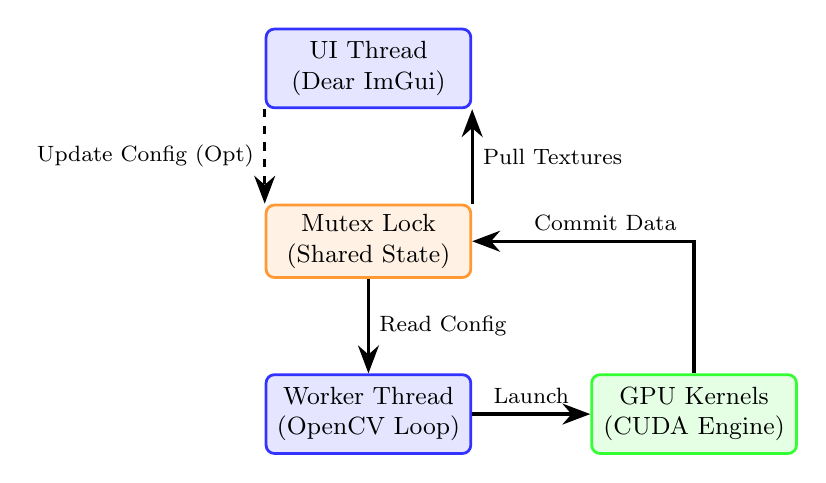
\begin{tikzpicture}[
    node distance=1.2cm and 1.5cm,
    block/.style={rectangle, draw, rounded corners=3, fill=blue!10, draw=blue!80, line width=1pt, minimum width=2.6cm, minimum height=1cm, align=center, font=\small},
    mutex/.style={rectangle, draw, rounded corners=3, fill=orange!10, draw=orange!80, line width=1pt, minimum width=2.6cm, minimum height=0.8cm, align=center, font=\small},
    gpu/.style={rectangle, draw, rounded corners=3, fill=green!10, draw=green!80, line width=1pt, minimum width=2.6cm, minimum height=1cm, align=center, font=\small},
    line/.style={-{Stealth[scale=1.2]}, line width=1.2pt},
    optline/.style={-{Stealth[scale=1.2]}, line width=1.2pt, dashed}
]
    % Layout
    \node[block] (UI) {UI Thread\\(Dear ImGui)};
    \node[mutex, below=of UI] (Mutex) {Mutex Lock\\(Shared State)};
    \node[block, below=of Mutex] (Worker) {Worker Thread\\(OpenCV Loop)};
    \node[gpu, right=of Worker] (GPU) {GPU Kernels\\(CUDA Engine)};

    % Arrows
    \draw[optline] (UI.south west) -- (Mutex.north west) node[midway, left, font=\footnotesize] {Update Config (Opt)};
    \draw[line] (Mutex.north east) -- (UI.south east) node[midway, right, font=\footnotesize] {Pull Textures};
    \draw[line] (Mutex) -- (Worker) node[midway, right, font=\footnotesize] {Read Config};
    \draw[line] (Worker) -- (GPU) node[midway, above, font=\footnotesize] {Launch};
    \draw[line] (GPU.north) |- (Mutex.east) node[pos=0.7, above, font=\footnotesize] {Commit Data};
\end{tikzpicture}%
}
\caption{Dual-Threaded Architecture with Asynchronous CUDA Pipeline Staging}
\label{fig:system_architecture}
\end{figure}

The UI Thread handles the window event loop and renders the immediate-mode Dear ImGui panels \cite{ImGui}. The Worker Thread runs the active clustering solver, looping through BGR frame acquisition via OpenCV \cite{Bradski2000}, CUDA-based distance calculation \cite{CudaGuide}, and direct GPU pixel re-coloring. This asynchronous boundary isolates computational latency from frame display pacing.

\subsection{Object-Oriented Design Patterns}
To maintain modularity, the system integrates several standard software engineering design patterns:
\begin{itemize}
    \item \textbf{Strategy Pattern:} Solvers are structured around the abstract \texttt{KMeansEngine} class. The \texttt{ClassicalEngine} and \texttt{QuantumEngine} act as interchangeable strategies, allowing live hot-swapping \cite{gamma1995design}.
    \item \textbf{Factory Method:} The \texttt{ClusteringFactory} instantiates the solver and centroid initialization variants based on configuration enums \cite{gamma1995design}.
    \item \textbf{Facade Pattern:} The \texttt{ClusteringManager} exposes a clean interface to hide raw preprocessing, kernel execution, and VRAM mapping operations \cite{gamma1995design}.
    \item \textbf{RAII (Resource Acquisition Is Initialization):} The \texttt{CudaAssignmentContext} controls memory allocation and release, ensuring device buffers are automatically freed during runtime layout adjustments \cite{stroustrup2022tour}.
    \item \textbf{Bridge Pattern (Pimpl):} Used in the manager classes as a compiler firewall to isolate CUDA and OpenCV includes from the global project compilation scope \cite{meyers2014effective}.
\end{itemize}

\subsection{Data Normalization and Preprocessing}
Pixels are converted into BGR features normalized to $[0, 1]$ and spatial features normalized by the frame dimensions: $\mathbf{x}_n = [B_n, G_n, R_n, \lambda_{\text{spatial}} x_n, \lambda_{\text{spatial}} y_n]^T$, with $\lambda_{\text{spatial}} = 10^{-6}$ \cite{shi2000normalized, achanta2012slic}. Centroid estimation is performed on a subsampled sparse manifold by stride sampling the frame at spatial stride $S \in [1, 16]$. By the Law of Large Numbers, this uniform sampling retains representation while reducing complexity by a factor of $S^2$ \cite{mouton2020stride}.

Thread communication is orchestrated through a thread-safe mutex bridge using \texttt{std::mutex} and \texttt{std::scoped\_lock} \cite{williams2019c++}, preventing race conditions when hot-swapping hyperparameters or transferring final textures (see Fig.~\ref{fig:system_architecture}).

\section{Implementation and Optimization}
Detail the CUDA kernel details, downsampling, and memory layouts (AoS vs. SoA) here.

\section{Experimental Results and Discussion}\label{sec:results}
To evaluate the performance of the GPU-accelerated C++/CUDA framework, we conduct comparative latency profiling, convergence analysis, and quantitative quality benchmarking between the classical Euclidean and quantum-inspired engines.

\subsection{Experimental Environment and Methodology}
All benchmarks are executed on a local system with an Intel Core Ultra 9 275HX CPU, 32~GB RAM, and an NVIDIA GeForce RTX 5070 Ti GPU (12~GB VRAM) under Windows 11. To ensure fair and reproducible comparisons, a global fixed-seed protocol (\texttt{STABLE\_RANDOM\_SEED = 42}) is implemented across the Mersenne Twister (\texttt{std::mt19937}) random initialization and the Monte Carlo silhouette sampling logic. Mathematical correctness is verified via a comprehensive GoogleTest suite targeting boundary conditions, empty cluster resilience, and CPU-GPU numerical parity (maintaining a $10^{-5}$ tolerance under floating-point drift).

\subsection{Latency Profiling and Throughput Scaling}
The system's execution latency is profiled across three standard operational modes under live camera processing: Performance ($K=3$, $S=8$), Balanced ($K=8$, $S=4$), and High Quality ($K=40$, $S=1$), where $K$ is the cluster count and $S$ is the downsampling stride. Table~\ref{tab:telemetry} details the stage-level latencies averaged over 21 runs.

\begin{table}[t]
\centering
\footnotesize
\caption{System Performance and Stage Latency Telemetry}
\label{tab:telemetry}
\begin{tabular}{ccccc}
\hline
\textbf{Mode} & \textbf{Preprocess} & \textbf{Optimize} & \textbf{Assign} & \textbf{Total Latency} \\ \hline
Performance  & 0.28 ms & 0.47 ms & 0.59 ms & \textbf{1.33 ms} \\
Balanced     & 0.29 ms & 0.74 ms & 0.59 ms & \textbf{1.62 ms} \\
High Quality & 0.30 ms & 2.93 ms & 0.62 ms & \textbf{3.86 ms} \\ \hline
\end{tabular}
\end{table}

The preprocessor kernel executes in $\approx 0.29\text{ ms}$ regardless of parameters due to 2D grid index efficiency. Centroid learning (optimization) scales with the active pixel count (stride $S$) and cluster count $K$, while pixel assignment scales minimally due to parallel thread occupancy. Across all modes, the pipeline achieves theoretical throughputs of $750\text{ FPS}$ (Performance), $618\text{ FPS}$ (Balanced), and $259\text{ FPS}$ (High Quality), vastly exceeding the real-time target of $120\text{ FPS}$ ($8.33\text{ ms}$ frame budget) and leaving substantial processing headroom under live 30 FPS video feeds.

Table~\ref{tab:latency_benchmarks} evaluates average execution latency and convergence iteration counts under a highly textured static workspace over 21 trials (using K-Means++ seeding) to evaluate GPU scaling under heavy workloads.

\begin{table}[b]
\centering
\small
\caption{Performance Comparison of Classical vs. Quantum K-Means}
\label{tab:latency_benchmarks}
\begin{tabular}{ccccc}
\hline
\textbf{Mode} & \multicolumn{2}{c}{\textbf{Classical}} & \multicolumn{2}{c}{\textbf{Quantum}} \\
 & \textbf{Lat. (ms)} & \textbf{Iter.} & \textbf{Lat. (ms)} & \textbf{Iter.} \\ \hline
Performance  & 1.8056  & 11.71  & 1.6107  & 12.38  \\
Balanced     & 6.4545  & 41.81  & 6.1547  & 41.43  \\
High Quality & 26.6608 & 88.67  & 27.9470 & 88.62  \\ \hline
\end{tabular}
\end{table}

Under low-density and balanced loads, the quantum-inspired engine is slightly faster ($1.61\text{ ms}$ vs. $1.81\text{ ms}$ and $6.15\text{ ms}$ vs. $6.45\text{ ms}$). This is driven by SFU hardware-accelerated cosine intrinsics. Under high density ($K=40, S=1$), the classical engine is slightly faster ($26.66\text{ ms}$ vs. $27.95\text{ ms}$). Despite trigonometric calculations, the engines maintain near-parity due to global VRAM fetch latencies dominating overall execution, allowing the GPU to hide arithmetic overhead by scheduling warps.

\subsection{Quantitative Clustering Quality and Lighting Telemetry}
Clustering quality was evaluated on a static VGA frame under two illumination environments: Scene A (uniform studio lighting) and Scene B (dim room with monitor glow and high sensor noise). Table~\ref{tab:quality_metrics} details the quality diagnostics under the balanced configuration ($K=8$, $S=4$, 21-run average).

\begin{table}[t]
\centering
\footnotesize
\caption{Segmentation Quality and Telemetry under Varying Lighting}
\label{tab:quality_metrics}
\setlength{\tabcolsep}{4pt}
\begin{tabular}{lccccc}
\hline
\textbf{Engine} & \textbf{Lat. (ms)} & \textbf{Iter.} & \textbf{WCSS} & \textbf{$\mathcal{D}\mathcal{B}$} & \textbf{Sil.} \\ \hline
\multicolumn{6}{l}{\textbf{Scene A (Studio)}} \\
\quad Classical & 5.4841 & 36.48 & 2189.43 & 0.68200 & 0.48335 \\
\quad Quantum   & 5.3617 & 35.81 & 2189.49 & 0.68194 & 0.48338 \\ \hline
\multicolumn{6}{l}{\textbf{Scene B (Low-Light)}} \\
\quad Classical & 2.7696 & 18.38 & 711.41  & 0.65632 & 0.54520 \\
\quad Quantum   & 2.9941 & 18.33 & 711.42  & 0.65636 & 0.54527 \\ \hline
\end{tabular}
\end{table}

The quantum-inspired engine achieves mathematical parity with the classical Euclidean solver: WCSS differs by less than $0.003\%$, while the Davies-Bouldin index and Silhouette scores align within $10^{-4}$. This is because the cosine-squared mapping remains monotonic within $[0, \pi/4]$, preserving the relative ordering of feature distances and converging to the same local minima. Thus, the non-linear Hilbert phase space mapping is a mathematically robust alternative that does not degrade class discrimination under noisy conditions.

\subsection{Visual Quality and Temporal Stability}
Full-frame segmentations (shown in Fig.~\ref{fig:case_study_1}) verify that both backends produce visually identical segment boundaries under both studio and low-light conditions.

\begin{figure}[b]
\centering
\begin{minipage}{0.32\columnwidth}
  \centering
  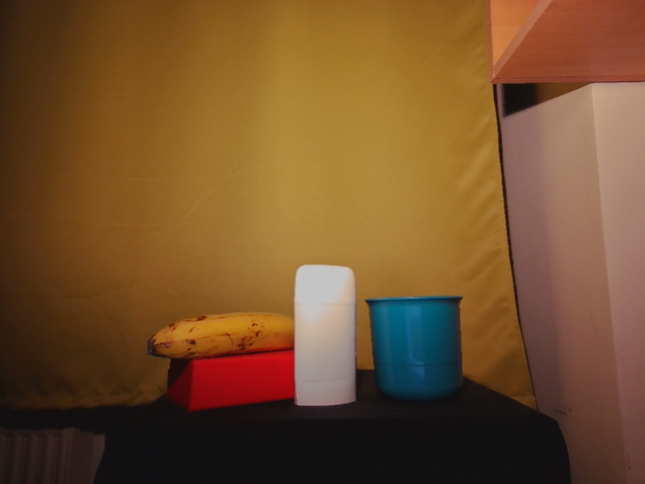
\includegraphics[width=\textwidth]{figures/scene_a.png}
  \vspace{0.1em}
  {\scriptsize Original (A)}
\end{minipage}\hfill
\begin{minipage}{0.32\columnwidth}
  \centering
  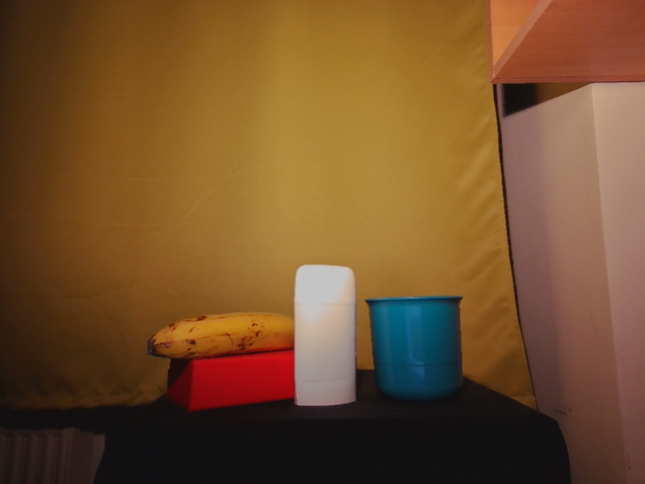
\includegraphics[width=\textwidth]{figures/scene_a.png}
  \vspace{0.1em}
  {\scriptsize Classical (A)}
\end{minipage}\hfill
\begin{minipage}{0.32\columnwidth}
  \centering
  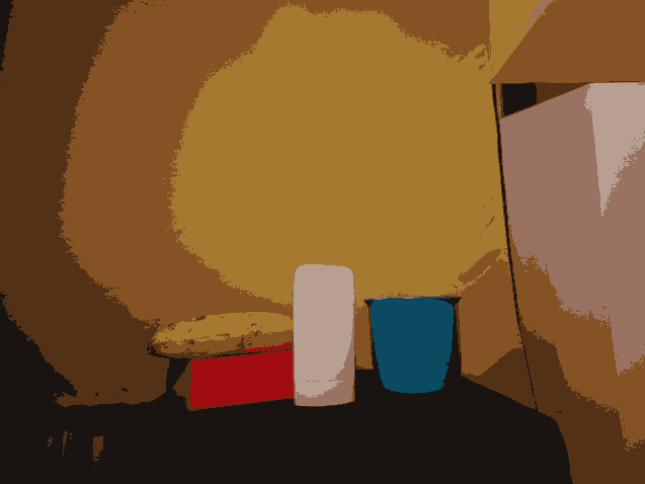
\includegraphics[width=\textwidth]{figures/scene_a_quantum.png}
  \vspace{0.1em}
  {\scriptsize Quantum (A)}
\end{minipage}

\vspace{0.3em}

\begin{minipage}{0.32\columnwidth}
  \centering
  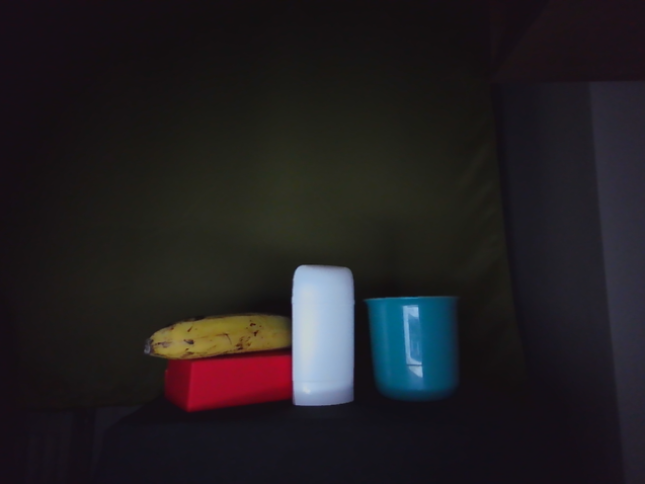
\includegraphics[width=\textwidth]{figures/scene_b.png}
  \vspace{0.1em}
  {\scriptsize Original (B)}
\end{minipage}\hfill
\begin{minipage}{0.32\columnwidth}
  \centering
  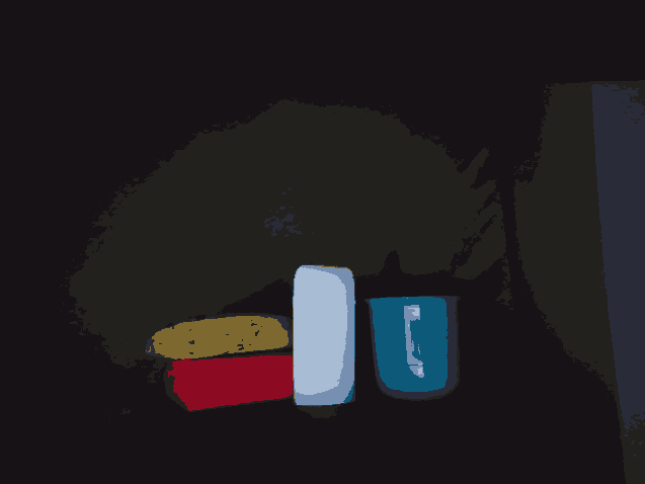
\includegraphics[width=\textwidth]{figures/scene_b_classical.png}
  \vspace{0.1em}
  {\scriptsize Classical (B)}
\end{minipage}\hfill
\begin{minipage}{0.32\columnwidth}
  \centering
  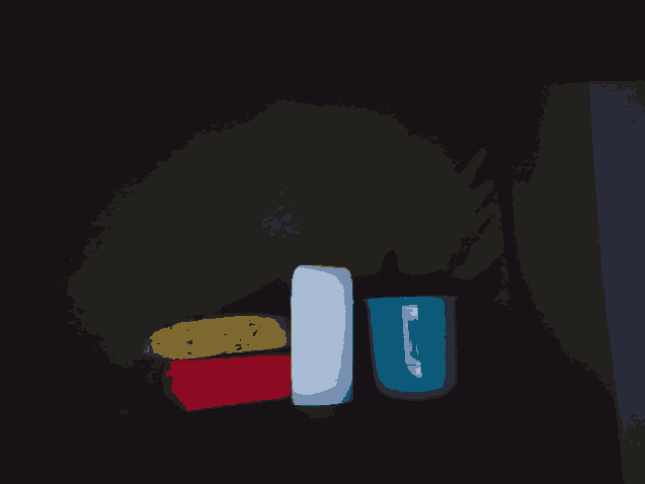
\includegraphics[width=\textwidth]{figures/scene_b_quantum.png}
  \vspace{0.1em}
  {\scriptsize Quantum (B)}
\end{minipage}
\caption{Visual Segmentations for Scenes A and B ($K=8$, $S=4$)}
\label{fig:case_study_1}
\end{figure}

The spatial weight parameter ($\lambda_{\text{spatial}} = 10^{-6}$) acts as a regularizer. Setting it too low allows color sensor noise to dominate and fragment clusters, whereas setting it too high forces grid-like partitions that ignore contours. The balanced spatial weighting prevents boundary noise while preserving sharp edge details in both backends. 

Under live video loops, frame-by-frame independent clustering results in temporal jitter. Jitter sequences reveal that random variations in initialization seeding cause both engines to allocate clusters differently between consecutive frames (e.g., shifting cluster assignments on flat background regions, which reduces the centroids available for resolving fine foreground detail). This identical shift confirms that temporal consistency is dominated by initial seeding strategies rather than the underlying metric topography.

\section{Conclusion and Future Work}\label{sec:conclusion}
This paper presented a high-throughput, GPU-accelerated C++/CUDA framework for real-time 5D image and video segmentation on a joint color-spatial manifold. By optimizing grid occupancy, utilizing on-chip shared memory atomics, and staging memory transfers through pinned DMA channels, the pipeline achieves theoretical throughputs up to $750\text{ FPS}$ on an RTX 5070 Ti, operating with significant headroom under the $120\text{ FPS}$ ($8.33\text{ ms}$) budget constraint.

The quantum-inspired engine emulates the multi-qubit state overlap of the quantum SWAP test by mapping pixel coordinates to phase states. Due to the monotonic nature of the cosine-squared mapping over the $[0, \pi/4]$ phase range, the quantum-inspired backend achieves visual and mathematical equivalence to the classical Euclidean solver under varying illumination conditions. Leveraging SFU hardware-accelerated math intrinsics (\texttt{\_\_cosf()}) bypasses standard ALU emulation, maintaining execution latency parity with classical Euclidean K-Means.

Future work will focus on integrating spatiotemporal constraints (such as Hungarian association or optical flow) to stabilize boundary jitter in continuous video streams. Additionally, we plan to port the phase-space similarity metrics to native NISQ hardware to evaluate real state-preparation and measurement delays under hardware noise, and optimize execution profiles on low-wattage embedded architectures.


\bibliographystyle{IEEEtran}
\bibliography{references}

\end{document}
